\chapter{集合と写像}
\label{chp:set}
 現代の数学において,集合と写像は
 欠かすことのできない「ことば」である.
 ここでは,集合の記法や演算について述べ,
 その性質を調べていく.
 後半では集合を使って写像を定義し,
 いくつかの基本的事項を述べる.

 本書で展開する集合論は
 {\index[widx]{そぼくしゅうごうろん@素朴集合論 \, naive set theory}}
 \emph{素朴集合論}(naive set theory)
 と呼ばれており,集合論がうまれた初期になされた議論である.
 素朴集合論ではいくつかのパラドックスが見つかっており,
 そのパラドックスを回避すべく
 公理をもとに積み上げられた集合論を
 \index[widx]{こうり@公理 \, axiom!こうりてきしゅうごうろん@---的集合論 \, ---atic set theory}
 \emph{公理的集合論}(axiomatic set theory)という.
 そのため,素朴集合論においては
 厳密な議論がなされているとは言い難い箇所がある.
 とはいえ,公理的集合論を
 理解するためには素朴集合論を理解するのが
 手っ取り早いこと,
 集合論を他分野に応用することを踏まえれば
 素朴集合論で十分なことも多いことを考慮し,
 素朴集合論のみを解説する.
%
%
%
%
%
 \section{集合とその記法}
 \label{sec:set}
 \paragraph{集合}
 範囲のはっきりした「モノ」の集まりを
 \index[widx]{しゅうごう@集合 \, set}
 \emph{集合}(set)といい,
 集合を構成する「モノ」のことをその集合の
 \index[widx]{ようそ@要素 \, element|see{元}} %
 \emph{要素} もしくは
 \index[widx]{げん@元 \, element}
 \emph{\ruby{元}{ゲン}}(element)という.
 対象$a$が集合$A$の元であることを$a$は$A$に
 \index[widx]{ぞくする@属する \, belong to}
 \emph{属する}(belong to)といい,
 \begin{align}
   a \in A
   \label{eq:setelement}
 \end{align}
 と表す
 \footnote{「属する」の代わりに,あるいは同じ意味の言葉として
           「含む」,「含まれる」という言葉が使われることがあるが,
            誤解が生じるのを防ぐため,
            本書では「属する」と「含む」は明確に区別して用いる.}
 .
 また,集合$A$と対象$a$について,条件$\lnot (a  \in A)$は
 \begin{align}
   a \notin A
   \label{eq:setelementnot}
 \end{align}
 と略記される.これは,「$a$は$A$の元ではない」
 という意味である.
 \begin{ex} \label{ex:setrei}
   「自然数全体の集まり」は集合である.これを通常$\mathbb{N}$と表す.
   条件$n \in \mathbb{N}$は「$n$は自然数である」ことを表す.

   一方,「背の高い人の集まり」や「大きい三角形の集まり」
   はどの対象が元であるかの範囲がはっきりせず,集合ではない.
 \end{ex}

 2つの集合$A,  B$について,$A$の元すべてが$B$の元でもある,
 すなわち,
 \begin{align*}
   \forall x (x \in A \to x \in B)
 \end{align*}
 が成り立つとき,$A$は$B$の
 \index[widx]{しゅうごう@集合 \, set!ぶぶん@部分--- \, subset}
 \emph{部分集合}(subset)
 である,もしくは$B$は$A$を
 \index[widx]{ふくむ@含む \, contain}
 \emph{含む}(contain)といい,
 \begin{align}
   A \subset B
   \label{eq:defsubset}
 \end{align}
 と表す.
 集合$A,  B$に対し,条件$\lnot ( A \subset B )$は
 \begin{align}
   A \not\subset B 
   \label{eq:nsubset}
 \end{align}
 と略記される.

 また,2つの集合$A,  B$について,$A \subset B$と$B \subset A$がともに成り立つ,
 すなわち,
 \begin{align*}
   \forall x (x \in A \rightleftarrows x \in B)
 \end{align*}
 が成り立つとき,
 $A$と$B$は集合として \emph{等しい}(equal)といい,
 \begin{align}
   A = B
   \label{eq:setequal}
 \end{align}
 と書き表す.このことは,集合がその元によってのみ決定されることを表している.
 
 2つの集合$A,  B$について,$A \subset B$かつ$A \neq B$であるとき,
 $A$は$B$の
 \index[widx]{しゅうごう@集合 \, set!しんぶぶん@真部分--- \, proper subset}
 \emph{真部分集合}(proper subset)であるといい,
 \begin{align}
   A \subsetneq B
   \label{eq:propersubset}
 \end{align}
 と表す
 \footnote{集合$A,  B$について,$A$が$B$の部分集合であることを
           $A \subseteq B$と表し,$A$が$B$の真部分集合であることを
           $A \subset B$と表す場合もあるが,現在ではあまり用いられない.}
 .
 
 2つの集合$A,  B$に対し,$A \subset B$か$B \subset A$のいずれかが成り立つとき,
 $A$と$B$には
 \index[widx]{ほうがんかんけい@包含関係 \, inclusion relation}
 \emph{包含関係}(inclusion relation)があるという.

 \begin{thm} \label{thm:hougansuii}
   3つの集合$A,  B,  C$に対し,
   $A \subset B$かつ$B \subset C$であれば$A \subset C$である.
 \end{thm}
 \begin{proof}
   $x \in A$を任意にとると,$A \subset B$であるから$x \in B$となり,
   $B \subset C$であるから$x \in C$となる.
   従って,$\forall x ( x \in A \to x \in C)$
   が成り立つので$A \subset C$となる.
 \end{proof}

 \paragraph{外延的記法と内包的記法}
 集合は,その元によってのみ決定されるのであった.
 従って,集合を表現するにはその元を明示すればよい.

 集合の表し方は2種類ある.1つ目はその元をすべて書き並べる方法で,
 \index[widx]{がいえんてききほう@外延的記法 \, extension notation}
 \emph{外延的記法}(extension notation)と呼ばれている.
 外延的記法では,集合は$\Set{ (\text{集合の元}) }$という形で表される.
 \begin{ex} \label{ex:gaienkihou}
   $1,  2,  3,  4$の4つの元からなる集合は,外延的記法で
   \begin{align*}
     \Set{ 1,  2,  3,  4}
   \end{align*}
   と表される.
   また,1から100までの自然数全体の集合は,
   その元を愚直に書いていてはとても書ききれないので
   「$\ldots$」を使って
   \begin{align*}
     \Set{ 1,  2,  \ldots , 100}
   \end{align*}
   と表す.これも外延的記法である.明らかに
   \begin{align*}
     \Set{ 1,  2,  3,  4} \subset \Set{ 1,  2,  \ldots ,  100}
   \end{align*}
   が成り立つ.
   自然数全体の集合$\mathbb{N}$や整数全体の集合$\mathbb{Z}$は,
   外延的記法では
   \begin{align*}
     \mathbb{N} & =\Set{ 1,  2,  \ldots } \\
     \mathbb{Z} & = \Set{ \ldots ,  -2 ,  -1 , 0 ,  1,  2,  \ldots}
   \end{align*}
   のように表される.
   $\mathbb{Z}$に関しては
   \[
     \mathbb{Z} = \Set{ 0, \pm 1, \pm 2,  \ldots }
   \]
   と表記されることも多い.
   \begin{align*}
     \Set{ 1,  2,  3,  4} \subset \Set{ 1,  2,  \ldots ,  100}
     \subset \mathbb{N} \subset \mathbb{Z}
   \end{align*}
   が成り立つことは容易にわかる.
  
 \end{ex}
 \begin{ex} \label{ex:settyouhuku}
   集合$\Set{ 1,  2,  3,  4}$と集合$\Set{ 2,  1,  1,  4,  3,  4}$
   は等しい.
   集合を考えるときにはその元の並び順や重複は考慮せず,
   元の種類のみを考える.
 \end{ex}
 
 ある「モノ」の集まりが集合であるかどうかははっきりしているから,
 集合を構成する「モノ」は集合であってもよい.
 \begin{ex} \label{ex:setofset}
   2つの集合$\Set{ 1,  2},  \Set{3,  4}$の相異なる元の個数の合計は
   4であるが,これら2つの集合を元とする集合$\Set{ \Set{ 1,  2} ,  \Set{3,  4}}$
   の元の個数は2である.また,
   \begin{align*}
     \Set{ 1,  2} \in \Set{ \Set{1,  2} ,  \Set{3,  4}} \\
     \Set{ \Set{1,  2}} \subset \Set{ \Set{1,  2} ,  \Set{ 3,  4}}
   \end{align*}
   などが成り立つ.
 \end{ex}

 もう1つの集合の表し方は,集合の元が満たすべき条件を与える方法であり,
 \index[widx]{ないほうてききほう@内包的記法 \, intension notation}
 \emph{内包的記法}(intension notation)と呼ばれている.
 変数$x$の条件$P(x)$について,$P(x)$を満たす$x$全体の集合を
 \begin{align}
   \Set{ x \mid  P(x) }
   \label{eq:naihouset}
 \end{align}
 と表す
 \footnote{この形の集合をすべて集合として認めると不都合が起こることがわかっているのだが,
           ここではそれは考えないことにする.
         本来「内包的記法」と呼ばれるべき集合の表し方は式\eqref{eq:naihousetS}の方である.}
   .
 また,変数$x$の条件$P(x)$と集合$S$について,
 集合
 \begin{align*}
   \Set{ x \mid  x \in S \land P(x) }
 \end{align*}
 を
 \begin{align}
   \Set{ x \in S \mid  P(x)}
   \label{eq:naihousetS}
 \end{align}
 と略記する.さらに,関数記号$f$と$x$の条件$P(x)$に対し,集合
 \begin{align*}
   \Set{ y \mid  \exists x ( y=f(x)  \land P(x)) } 
 \end{align*}
 のことを
 \begin{align}
   \Set{ f(x) \mid  P(x) }
   \label{eq:functionryakki}
 \end{align}
 と略記することがある.
 \begin{ex} \label{ex:naihou}
0以上1以下の実数全体の集合を$[ 0, 1]$と表すと,この集合は内包的記法で
   \begin{align*}
     [ 0,1] & = \Set{ x \mid  x \in \mathbb{R} \land 0 \leq x \leq 1} \\
            & = \Set{ x \in \mathbb{R} \mid  0 \leq x \leq 1}
   \end{align*}
   と表せる.
   また,偶数全体の集合を$2 \mathbb{Z}$と表すと,$2 \mathbb{Z}$は内包的記法で
   \begin{align*}
     2 \mathbb{Z} & = \Set{ x \mid  \exists n \in \mathbb{Z} ( x = 2n) } \\
                  & = \Set{ 2n \mid  n \in \mathbb{Z} }
   \end{align*}
   などと表せる.条件は数式で表現しなければならないわけではなく,
   \begin{align*}
     2 \mathbb{Z} = \Set{ x \mid  \text{$x$は偶数}}
   \end{align*}
   などと表してもよい.
   また,
   \[
     \Set{ x \mid P(x) \land Q(x) }
   \]
   の形をした集合は
   \[
     \Set{ x \mid P(x) , Q(x) }
   \]
   と表記されることも多い.
 \end{ex}
 内包的記法で集合を表すときに使う変数は仮の変数,
 すなわち束縛変数である.
 従って,内包的記法で集合を表すとき,
 どのような記号を用いるかは自由であり,
 違う記号に取り替えても表す集合は変わらない.
 \begin{ex} \label{ex:naihousokubaku}
   集合$A,B, C,D$を
   \begin{align*}
     A & = \Set{ y \mid \exists n \in \mathbb{N} (y=2n) }, \\
     B & = \Set{ t \mid \exists n \in \mathbb{N} (t=2n) }, \\
     C & = \Set{ n \mid \exists m \in \mathbb{N} (n = 2m) } , \\
     D & = \Set{ 2n \mid n \in \mathbb{N} }
   \end{align*}
   と定めたとき,$A,B,C,D$はすべて等しい.
   これらの集合はすべて$2 \mathbb{Z}$を表す.
 \end{ex}
 \begin{ex} \label{ex:kukan}
   $a<b$を満たす実数$a,  b$に対し,2つの集合$[a,b]$と$(a,b)$を
   \begin{align}
     [a,b] & = \Set{x \in \mathbb{R} \mid  a \leq x \leq b} ,
     \label{eq:heikukan} \\
     (a,b) & = \Set{ x \in \mathbb{R} \mid  a < x < b}
     \label{eq:kaikukan}
   \end{align}
   と定める.$a<b$となる実数$a,  b$を用いて$[a,b]$という形で表される集合を
   \index[widx]{へいくかん@閉区間 \, closed interval}
   \emph{閉区間}(closed interval)といい,
   $(a,b)$という形で表される集合を
   \index[widx]{かいくかん@開区間 \, open interval}
   \emph{開区間}(open interval)という.
   閉区間$[a,b]$に対し,区間の端の値$a,  b$はこの区間の
   \index[widx]{たんてん@(区間の)端点 \, endpoints}
   \emph{端点}(endpoints)と呼ばれることがある.

   また,$a<b$となる実数$a,b$について,集合$[a,b),  (a,b]$を
   \begin{align}
     [a,b) & = \Set{ x \in \mathbb{R} \mid  a \leq x < b},
     \label{eq:hankaikukanhidari} \\
     (a,b] & = \Set{ x \in \mathbb{R} \mid  a < x \leq b}
     \label{eq:hankaimigi}
   \end{align}
   と定め,この形で表される集合を
   \index[widx]{はんかいくかん@半開区間 \, half-open interval}
   \emph{半開区間}(half-open interval)
   という.

   閉区間,開区間,半開区間を総称して
   \index[widx]{ゆうげんくかん@有限区間 \, finite interval}
   \emph{有限区間}(finite interval)
   という.

   さらに,実数$a$に対して4つの集合$( - \infty , a],  ( -\infty , a)$
   および$[a, + \infty ),  (a, + \infty )$を
   \begin{align}
     (- \infty  , a ] & = \Set{ x \in \mathbb{R} \mid  x \leq a},
     \label{eq:mugenmigileq} \\  
     (- \infty  , a ) & = \Set{ x \in \mathbb{R} \mid  x < a},
     \label{eq:mugenmigi} \\
     [a, + \infty ) & = \Set{ x \in \mathbb{R} \mid  a \leq x},
     \label{eq:mugenhidarileq} \\
     (a,+ \infty ) & = \Set{ x \in \mathbb{R} \mid  a < x}
     \label{eq:mugenhidari} 
   \end{align}
   と定め,この形で表される集合
   を総称して
   \index[widx]{むげんくかん@無限区間 \, infinite interval}
   \emph{無限区間}(infinite interval)
   という.
 \end{ex}
   集合を考える上では,「元をもたない集合」を考えると都合がよい.
   この「元をもたない集合」を
   \index[widx]{しゅうごう@集合 \, set!くう@空--- \, empty set}
   \emph{\ruby{空}{クウ}集合}(empty set)といい,
   $\varnothing$と表す
   \footnote{空集合を表す記号$\varnothing$とギリシャ文字$\phi$は
             よく似ていて紛らわしいが,まったくの別物である.
             $\varnothing$はノルウェー文字をもとにした記号である.}
   .
  空集合$\varnothing$は任意の$x$に対し$x \notin \varnothing$を満たす集合である. 
  空集合は外延的記法で$\varnothing = \set{ }$と表すこともできる.

    
   \begin{que} \label{que:varnothing}
     空集合はすべての集合の部分集合であることを示せ.
     また,空集合の部分集合は自身に限られることを示せ.
   \end{que}

   問\ref{que:varnothing}により,任意の$x$に対して$x \notin A$を満たす集合$A$は
   ただ1つであることがわかる(のでこの唯一の集合を$\varnothing$と表記している).
  


   % 

 \section{集合の演算}
 \label{sec:enzan}

   ここからは,与えられた集合を用いて新しい集合を構成することを考える.

  \paragraph{和集合と共通部分}
   2つの集合$A,  B$について,集合$A \cup B$を
   \begin{align}
     A \cup B = \Set{ x \mid  x \in A \lor x \in B}
     \label{eq:union}
   \end{align}
   と定め,これを$A$と$B$の
   \index[widx]{しゅうごう@集合 \, set!わしゅうごう@和--- \, union}
   \emph{和集合}(union)という.
   記号「$\cup$」は「カップ」と読むことが多い.
   集合$A,  B$に対し,$A \cup B = B \cup A$が成り立つことは明らかであろう.
   
   \begin{ex} \label{ex:union}
     2つの集合$\Set{ 1,  2},  \Set{ 2,  3}$に対し,
     その和集合は$\Set{ 1,  2} \cup \Set{ 2,  3} = \Set{1,  2,  3}$である.
     また,2つの集合$\Set{\Set{1,  2}} ,  \Set{ 1,  2}$に対し,
     その和集合は
     $\Set{\Set{1,  2}} \cup \Set{1,  2} = \Set{ \Set{1,  2},  1,  2}$
     となる.
   \end{ex}
   
   2つの集合$A,  B$に対し,$A$と$B$の和集合$A \cup B$は
   $A$の元と$B$の元をすべて集めてできる集合である.
   
   \begin{thm} \label{thm:union}
     2つの集合$A,  B$に対し,
       $A \subset A \cup B , B \subset A \cup B$
     が成り立つ.
     また,集合$C$に対し,
       $A \subset C \text{かつ} B \subset C \text{ならば} A \cup B \subset C$
     となる.
   \end{thm}
   \begin{proof}
     直感的には明らかではあるが,定義に従って証明しよう.
     まず$A \subset A \cup B$
     を示す.
     $x \in A$を任意にとれば,$x \in A \lor x \in B$となるので
     $x \in A \cup B$となる.
     よって,$\forall x( x \in A \to x \in A \cup B)$となるので
     $A \subset A \cup B$が成り立つ.
     同様にして$B \subset A \cup B$も示せる.

     次に$C$が$A \subset C $かつ$B \subset C$を満たすとして,
     $A \cup B \subset C$となることを示す.
     $x \in A \cup B$を任意にとると,$x \in A \lor x \in B$である.
     $x \in A$の場合には$A \subset C$より$x \in C$であり,
     $x \in B$の場合には$B \subset C$より$x \in C$となる.
     いずれにしても$x \in C$が成り立つから,
     $\forall x (x \in A \cup B \to x \in C)$
     となり,$A \cup B \subset C$が成り立つ.
   \end{proof}
   定理\ref{thm:union}は,
   集合$A,  B$に対し,$A \cup B$が$A$と$B$の両方を含む
   集合の中で,包含関係について最小のものであることを示している.
   
   また,2つの集合$A,  B$に対し,集合$A \cap B$を
   \begin{align}
     A \cap B = \set{ x \mid  x \in A \land x \in B}
     \label{eq:kyoutuububun}
   \end{align}
   と定め,これを$A$と$B$の
   \index[widx]{きょうつうぶぶん@共通部分 \, intersection}
   \emph{共通部分}(intersection)という.
   記号「$\cap$」は通常「キャップ」と読む.
   和集合のときと同様に,集合$A,  B$に対し,$A \cap B = B \cap A$
   が成り立つ.
   
   \begin{ex} \label{ex:intersection}
     2つの集合$\set{1,  2,  3},  \set{2,  3,  4}$について,
     その共通部分は
     $\set{1,  2,  3} \cap \set{2,  3,  4} = \set{ 2,  3}$
     である.また,2つの集合$\set{1,  2} ,  \set{3,  4}$について,
     その共通部分は空である.すなわち,
     $\set{1,  2} \cap  \set{3,  4} = \varnothing$である.
   \end{ex}
   
   2つの集合$A,  B$について,その共通部分$A \cap B$は
   $A$と$B$両方に属している元全体の集合である.

   一般に,集合$A,  B$に対し,$A \cap B = \varnothing$であるとき,
   $A$と$B$は
   \index[widx]{たがいにそ@(集合が)互いに素 \, disjoint}
   \emph{互いに素}である,あるいは
   \index[widx]{まじわらない@交わらない \, disjoint|see{互いに素}} %
   \emph{交わらない}(disjoint)
   という.
   また,集合$A,  B$が互いに素であるとき,$A$と$B$の和集合を
   特に$A$と$B$の(集合論的)
   \index[widx]{ちょくわ@(集合論的)直和 \, direct sum}
   \emph{直和}(direct sum),
   あるいは
   \index[widx]{ひこうわ@非交和 \, disjoint union|see{直和}} %
   \emph{非交和}(disjoint union)といい,
   $A \sqcup B$と表すことがある.

   集合の共通部分に関しても,和集合と似た形式の定理が成り立つ.
   証明も同様である.
   \begin{thm} \label{thm:intersection}
     集合$A,  B$に対し,
       $A \cap B \subset A ,  A \cap B \subset B$
     が成り立つ.また,集合$C$について,
       $C \subset A \text{かつ} C \subset B \text{ならば} C \subset A \cap B.$
   \end{thm}
   
   定理\ref{thm:intersection}により,集合$A,  B$に対し,
   その共通部分$A \cap B$は$A$と$B$両方に含まれる集合のうち,
   包含関係に関して最大の集合であることがわかる.

   \begin{que} \label{que:unionintersection}
     集合$A,  B$を
     \begin{align*}
       A & = \set{n \in \mathbb{Z} \mid  n \text{は奇数} , \, 0<n<10}, \\ 
       B & = \set{ n \in \mathbb{Z} \mid  n \text{は3の倍数} , \, 0<n<15} 
     \end{align*}
     と定めたとき,$A \cup B$と$A \cap B$を外延的記法で表せ.
   \end{que}
   \begin{que} \label{que:naihouequal}
     集合$A,  B$を
     \begin{align*}
       A & = \Set{ x \in \mathbb{Z} \mid x \text{は素数} , \, 2<x<9} , \\
       B & = \Set{ x \in \mathbb{Z} \mid x \text{は奇数}, \, 2 \leq x \leq 7}
     \end{align*}
     と定めたとき,$A$と$B$の包含関係を調べよ.
   \end{que}
 

   問\ref{que:varnothing}の解答や定理\ref{thm:hougansuii},
   定理\ref{thm:union},
   および定理\ref{thm:intersection}の証明には
   命題論理と述語論理の性質を利用した.
   集合に対する$\cup ,  \cap ,  \subset ,  =$という記号と,
   命題(条件)に対する$\lor ,  \land ,  \to ,  \rightleftarrows$
   という記号はそれぞれ似た性質を示す.
   そのことを踏まえれば,以下の定理\ref{thm:unionintersection}
   は\ref{sec:sequent}で考察した関係を用いることで容易に証明できる.
   \begin{thm} \label{thm:unionintersection}
     3つの集合$A,  B,  C$に対し,
     \begin{align}
       (A \cup B ) \cup C & = A \cup (B \cup C) ,
       \label{eq:ketugoucap} \\
       (A \cap B) \cap C & = A \cap (B \cap C),
       \label{eq:ketugoucup} \\
       (A \cup B) \cap C & = ( A \cap C) \cup (A \cap C),
       \label{eq:bunpaicap} \\
       (A \cap B) \cup C & = ( A \cup C) \cap (A \cup C)
       \label{eq:bunpaicup}
     \end{align}
     が成り立つ.
   \end{thm}
   \begin{proof}
     式\eqref{eq:ketugoucap}を示す.任意の対象$x$に対し,
     \begin{align*}
       x \in (A \cup B) \cup C & \equiv x \in A \cup B \lor x \in C \\
       & \equiv ( x \in A \lor x \in B) \lor x \in C \\
       & \equiv x \in A \lor ( x \in B \lor x \in C) \\
       & \equiv x \in A \lor x \in B \cup C \\
       & \equiv x \in A \cup ( B \cup C) . 
     \end{align*}
     よって,$\forall x ( x \in ( A \cup B) \cup C \rightleftarrows x \in A \cup (B \cup C))$
     が成り立つので$(A \cup B) \cup C = A \cup (B \cup C)$が成り立つ.
     式\eqref{eq:ketugoucup}も同様である.

     次に,式\eqref{eq:bunpaicap}を示す.任意の対象$x$に対し,
     \begin{align*}
       x \in (A \cup B) \cap C & \equiv x \in (A \cup B) \land x \in C \\
                               & \equiv (x \in A \lor x \in B) \land x \in C \\
                               & \equiv (x \in A \land x \in C) \lor (x \in B \land x \in C) \\
                               & \equiv x \in A \cap C \lor x \in B \cap C \\
                               & \equiv x \in (A \cap C ) \cup (B \cap C) . 
     \end{align*}
     よって,$\forall x ( x \in (A \cup B) \cap C \rightleftarrows 
     x \in (A \cap C) \cup (B \cap C))$が成り立つので
              $(A \cup B) \cap C = (A \cap C) \cup (B \cap C)$となる.
      式\eqref{eq:bunpaicup}も同様である.
   \end{proof}
   式\eqref{eq:ketugoucap}と式\eqref{eq:ketugoucup}により,
   集合$A,  B,  C$に対して
   $A \cup B \cup C$や$A \cap B \cap C$などという記法が許されることがわかる.
    
   \paragraph{差集合}
   集合$A,  B$について,集合
   \begin{align}
     \set{ x \mid  x \in A \land x \notin B}
     \label{eq:differenceset}
   \end{align}
   を$A$と$B$の
   \index[widx]{しゅうごう@集合 \, set!さしゅうごう@差--- \, difference ---}
   \emph{差集合}(difference set)
   (より正確には$A$から$B$を引いた差集合)といい,
   $A -B$あるいは$A \setminus B$と表す.
   \begin{ex} \label{ex:setminus}
     集合$\set{1,  2,  3,  4,  5},  \set{3,  4,  8}$
     に対し,その差集合は
     $\set{1,  2,  3,  4,  5} - \set{3,  4,  8} = \set{1,  2,  5}$
     となる.
     また,実数全体の集合$\mathbb{R}$,有理数全体の集合$\mathbb{Q}$に対し,
     その差集合$\mathbb{R} - \mathbb{Q}$は無理数全体の集合を表す.
   \end{ex}

   集合$A,  B$に対し,その差集合$A-B$は$A$の元から$B$の元を
   「差し引いた」集合である.

   \paragraph{全体集合と補集合}
   数学理論においては,そのときに考えている集合がすべて,
   ある特定の集合$U$の部分集合であるということが少なくない.
   たとえば,微分積分学において,議論に現れる集合は
   ほとんどの場合実数全体の集合$\mathbb{R}$の部分集合である.
   そのような場合,議論の基礎となるその集合$U$のことを
   \index[widx]{しゅうごう@集合 \, set!ぜんたいしゅうごう@全体--- \, universal ---}
   \emph{全体集合}(universal set)という.

   全体集合$U$が与えられているとき,$U$の部分集合$A$について,
   $U$と$A$の差集合$U-A$はある意味で「$A$に属していない元全体の集合」
   を表すことになる.その意味で,集合$U-A$を
   $A$の
   \index[widx]{しゅうごう@集合 \, set!ほしゅうごう@補--- \, complementaly ---}
   \emph{補集合}(complementary set)といい,
   $A^c$と表す
   \footnote{高校の教科書では,集合$A$の補集合を$\overline{A}$
             と表すことが多いが,本書では用いない.}
   .
   \begin{ex} \label{ex:complement}
     全体集合$U$を整数全体の集合$\mathbb{Z}$と定めたとき,
     集合$A = \set{ 2n \mid  n \in \mathbb{Z}}$の補集合は
     $A^c = \set{ 2n-1 \mid  n \in \mathbb{Z}}$である.
   \end{ex}
   
   補集合に関して,次の定理\ref{thm:setdemorgan}は基本的で重要である.
   \index[widx]{De Morganのほうそく@De Morganの法則}
   \index[nidx]{De Morgan@De Morgan(ド・モルガン)}
   \begin{thm}[集合論におけるDe Morganの法則] \label{thm:setdemorgan}
     全体集合を$U$とし,$U$の部分集合$A,  B$に対して
     \begin{align}
       (A \cup B)^c & = A^c \cap B^c ,
       \label{eq:setdemorgancup} \\
       (A \cap B)^c & = A^c \cup B^c
       \label{eq:setdemorgancap}
     \end{align}
     が成り立つ.
   \end{thm}
   \begin{proof} 
     式\eqref{eq:setdemorgancup}を示す.任意の$x \in U$に対し,
     \begin{align*}
       x \in (A \cup B)^c & \equiv x \notin A \cup B \\
                          & \equiv \lnot( x \in A \cup B) \\
                          & \equiv \lnot (x \in A \lor x \in B) \\
                          & \equiv \lnot (x \in A) \land \lnot (x \in B) \\
                          & \equiv x \notin A \land x \notin B \\
                          & \equiv x \in A^c \land x \in B^c \\
                          & \equiv x \in A^c \cap B^c.
     \end{align*}
     よって,$\forall x \in U ( (A \cup B)^c \rightleftarrows x \in A^c \cap B^c)$
     が成り立つので$(A \cup B)^c = A^c \cap B^c$となる.
     式\eqref{eq:setdemorgancap}も同様に示せる.
   \end{proof}
   \begin{que} \label{que:univarseset}
     全体集合を$U$として,$A \subset U$について次の式が成り立つことを示せ.
     \begin{align}
       (A^c)^c = A,
       \label{eq:ccA} \\
       A \cup A^c = U, 
       \label{eq:AAcU} \\
       A \cap A^c = \varnothing ,
       \label{eq:AAcvarnothing} \\
       U^c = \varnothing ,
       \label{eq:Ucvarnothing} \\
       \varnothing ^c = U. 
       \label{eq:varnothingcU} 
     \end{align}
     また,$A,  B \subset U$に対し,
     \begin{align}
       A \subset B \equiv B^c \subset A^c
       \label{eq:settaiguu}
     \end{align}
     であることを示せ.
   \end{que}

  \paragraph{Venn図とEuler図}
   集合を平面上の円の内部と考え,
   その包含関係を視覚的に考察する方法を考える.

  \begin{figure}[h]
     \begin{minipage}[b]{0.45\linewidth}
       \centering
       \includegraphics[width=1.8cm]{inputyou/set/picture/seteulerdia.pdf}
       \subcaption{Eulerによる部分集合の表現} \label{fig:eulerdia}
     \end{minipage}
     \begin{minipage}[b]{0.45\linewidth}
       \centering
       \includegraphics[width=2.6cm]{inputyou/set/picture/setvenndia.pdf}
       \subcaption{Vennによる部分集合の表現} \label{fig:venndia}
     \end{minipage}
     \caption{部分集合の図による表現}
     \label{fig:eulervenndia}
   \end{figure}

   図\ref{fig:eulerdia}はEulerによる集合の表現の一例であり,
   集合$A$が集合$B$の部分集合であることを表している.
   Eulerの方法では,集合の包含関係を円が別の円の内部にあるかどうかで識別する.
   この方法で集合を表現した図を
   \index[widx]{Eulerず@Euler図 \, Euler digram}
   \index[nidx]{Euler@Euler(オイラー)}
   \textbf{Euler図}(Euler diagram)と呼ぶ.
   図\ref{fig:eulerdia}は$A$が$B$の真部分集合であることを表しているように見えるが,
   必ずしもそうとはいえないことに注意しなければならない.
   Eulerの方法では,集合$A$が集合$B$の部分集合であることと
   $A$が$B$の真部分集合であることを区別できない.
   
   図\ref{fig:venndia}はVennによる集合の表現の一例である.
   Vennの方法では,
   元が存在する領域をバツ印をつけて表現し,
   元が存在しない領域を斜線を引くことによって表現する.
   この方法で集合を表現した図を
   \index[widx]{Venn図@Venn図 \, Venn diagram} 
   \index[nidx]{Venn@Venn(ヴェン)}
   \textbf{Venn図}(Venn diagram)
   と呼ぶ.
   \begin{wrapfigure}{r}{2.8cm}
     \centering
     \includegraphics[width=2.5cm]{inputyou/set/picture/setvennproper.pdf}
     \caption{真部分集合の表現}
     \label{fig:propersubset}
   \end{wrapfigure}
   図\ref{fig:venndia}中の斜線が引かれた領域には元が存在しない,
   すなわち,$A$だけに属して$B$に属さない元が存在しないので,
   図\ref{fig:venndia}は集合$A$が
   集合$B$の部分集合であることを表現していることになる.

   Vennの方法では,$A$が$B$の真部分集合であることは
   図\ref{fig:propersubset}のように表される.
   斜線によって$A$のみに属し$B$に属さない元が存在しないことが表現され,
   $\times$によって$B$のみに属し$A$に属さない元が存在することが表現されている.
   このように,Vennの方法では領域が空であるか否かを明確に区別しようとしていることがわかる.

   ところが,現在「Venn図」といえばそれはEuler図のことを指していることがほとんどである.
   そして,図中の斜線は元が存在しないことを表現するのではなく,
   図中の領域を指定するのに使われることが多い.
   
   \begin{figure}[h]
     \begin{minipage}{0.3\linewidth}
       \centering
       \includegraphics[width=2.5cm]{inputyou/set/picture/setunion.pdf}
       \subcaption{和集合} \label{fig:setunion}
     \end{minipage}
     \begin{minipage}{0.3\linewidth}
       \centering
       \includegraphics[width=2.5cm]{inputyou/set/picture/setintersection.pdf}
       \subcaption{共通部分} \label{fig:setintersection}
     \end{minipage}
     \begin{minipage}{0.3\linewidth}
       \centering
       \includegraphics[width=2.5cm]{inputyou/set/picture/setvenndia.pdf}
       \subcaption{差集合} \label{fig:setdifference}
     \end{minipage}
     \caption{集合の演算の表現}
     \label{fig:setenzan}
   \end{figure}
   たとえば,集合$A,  B$に対し,その和集合$A \cup B$,
   共通部分$A \cap B$,差集合$A -B$はそれぞれ
   図\ref{fig:setunion},図\ref{fig:setintersection},図\ref{fig:setdifference}
   のように表される.
   これを応用すれば,図を用いて集合の分配律の成立を直感的に理解することができる.
   \begin{figure}[h]
     \begin{minipage}{0.45\linewidth}
       \centering
       \includegraphics[width=3cm]{inputyou/set/picture/setbunpaicap.pdf}
       \subcaption{分配律その1}
       \label{fig:setbunpaicap}
     \end{minipage}
     \begin{minipage}{0.45\linewidth}
       \centering
       \includegraphics[width=3cm]{inputyou/set/picture/setbunpaicup.pdf}
       \subcaption{分配律その2}
       \label{fig:setbunpaicup}
     \end{minipage}
     \caption{分配律の直感的理解}
     \label{fig:setbunpairitu}
   \end{figure}

   集合$A,  B,  C$に対し,集合$(A \cup B) \cap C$と
   $(A \cap C) \cup (B \cap C)$を図に表すと
   どちらも図\ref{fig:setbunpaicap}のようになり,
   これらの集合が等しいことがわかる.
   また,$(A \cap B) \cup C$と$(A \cup C) \cap (B \cup C)$
   を図に表すとともに図\ref{fig:setbunpaicup}のようになり,
   これらの集合が等しいことがわかる.

   \begin{wrapfigure}{r}{3.5cm}
     \centering
     \includegraphics[width=3cm]{inputyou/set/picture/setcomplement.pdf}
     \caption{補集合の表現}
     \label{fig:setcomplement}
   \end{wrapfigure}
   
   全体集合が定まっているときにはそれを長方形で表すことが多い.
   $U$を全体集合とする文脈において,集合$A$の補集合$A^c$は
   図\ref{fig:setcomplement}のようになる.
   この図から$A \cup A^c = U , \,  A \cap A^c = \varnothing$
   などが成り立つことが直感的に理解できる.

   集合論におけるDe Morganの法則の成立も
   図を用いて直感的に理解することができる.
   \begin{figure}[h]
     \begin{minipage}{0.45\linewidth}
       \centering
       \includegraphics[width=3cm]{inputyou/set/picture/setdemorgancup.pdf}
       \subcaption{De Morganの法則その1}
       \label{fig:setdemorgancup}
     \end{minipage}
     \begin{minipage}{0.45\linewidth}
       \centering
       \includegraphics[width=3cm]{inputyou/set/picture/setdemorgancap.pdf}
       \subcaption{De Morganの法則その2}
       \label{fig:setdemorgancap}
     \end{minipage}
     \caption{De Morganの法則の直感的理解}
     \label{fig:setdemorgan}
   \end{figure}
   
   全体集合を$U$とする文脈において,$A,  B \subset U$
   をとり,集合$(A \cup B)^c$と$A^c \cap B^c$を図に表すと
   どちらも図\ref{fig:setdemorgancup}のようになり,
   これらの集合が等しいことがわかる.
   さらに,$(A \cap B)^c$と$A ^c \cup B^c$を図に表せば
   どちらも図\ref{fig:setdemorgancap}のようになり,
   これらの集合が等しいことがわかる.

   Venn図による考察は万能であるかのように思われるが,
   実際には回転対称性を保ったままのVenn図が
   描けるのは,集合の数が素数のとき
   のみであることが知られている.


   \paragraph{順序対と直積集合}
   対象$a,  b$について,集合$\Set{ \Set{a} ,  \Set{a,  b}}$
   を$a$と$b$の
   \index[widx]{じゅんじょつい@順序対 \, orderd pair}
   \emph{順序対}(ordered pair),
   \index[widx]{つい@対 \, pair|see{順序対}}
   もしくは単に \emph{対} といい,$(a,b)$と表す.
   
   \begin{thm}[順序対の特徴づけ] \label{thm:orderedpair}
     対象$a,  b,  c,  d$に対し,
     $(a,b)=(c,d)$が成り立つための必要十分条件は,
     $a=c$かつ$b=d$となることである.
   \end{thm}
   \begin{proof}
     十分性が成り立つことは明らかであるから,必要性のみを示す.
     $(a,b) = (c,d)$とすると,
     \begin{align}
       \set{\set{a},  \set{a,b}} = \set{\set{c} ,  \set{c,  d}}
       \tag{$\ast$}
     \end{align}
     となる.$\set{ a } \in \set{ \set{a}, \set{a,b} }$
     だから$\set{a} \in \set{ \set{c} , \set{c,d}}$
     であり,$\set{a} = \set{c} $か
     $\set{a} = \set{c,d}$のどちらかが成り立つ.
     いずれにせよ$c \in \set{a}$となるので
     $a=c$である.このとき,式$(\ast)$は
     \begin{align}
       \set{\set{a} , \set{a,b}} = \set{\set{a} , \set{a,d}}
       \tag{$\ast\ast$}
     \end{align}
     となり,$\set{a,b} \in \set{\set{a},\set{a,d}}$
     であるから,$\set{a,b} = \set{a}$か
     $\set{a,b} = \set{a,d}$のいずれかが成り立つ.
     前者の場合は$a=b$より
     式$(\ast\ast)$の左辺が
     $\set{a}$となるから,$d=a=b$となる.
     後者の場合を考えよう.
     $b \in \set{a,d}$より$a=b$か$b=d$の
     いずれかであるが,
     どちらの場合も
     $b=d$が成り立つ.
     以上の議論により,$a=b$かつ$b=d$となることがわかる.
   \end{proof}

   定理\ref{thm:orderedpair}から次の事実がわかる.
   \begin{coro}
     対象$a,  b$について,$a \neq b$であれば$(a,b) \neq (b,a)$
     である.
   \end{coro}
   定理\ref{thm:orderedpair}とその系により,
   順序対は順序も考えた対象のペアであることがわかった.
   
   順序対の定義は定理\ref{thm:orderedpair}さえ成り立てば何でもよい.
   たとえば,対象$a,  b$に対し,その順序対$(a,b)$を
   \begin{align*}
     (a,b) & = \set{ \set{b},  \set{a,  b}}, \\
     (a,b) & = \set{ a,  \set{a,b}}
   \end{align*}
   などと定義しても定理\ref{thm:orderedpair}は成立する.
   従って,順序対の定義を上記のように変えても問題ないということになる.
   もっといえば,対象$a,  b$の順序対$(a,b)$を
   「定理\ref{thm:orderedpair}が成り立つような関数記号」
   として公理的に定義することも考えられる.

   順序対の引数を増やすことを考える.3つの対象$a_1,  a_2,  a_3$に対し,
   $a_1,  a_2,  a_3$の順序対$(a_1, a_2, a_3)$を
   $(a_1,a_2,a_3) = (a_1,(a_2,a_3))$と定めることにすると,
   この順序対も対象$a_1,  a_2,  a_3,  b_1,  b_2,  b_3$について,
   \begin{align*}
     (a_1,a_2,a_3) = (b_1,b_2,b_3) \equiv 
     a_1=b_1 \land a_2=b_2 \land a_3 = c_3
   \end{align*}
   を満たす.
   より一般に,$n$個の対象$a_1, a_2, \ldots ,  a_n$に対し,
   その順序対を$(a_1,a_2,\ldots ,a_n)=(a_1,(a_2,a_3,\ldots ,a_n)) $
   と$n-1$個の対象についての順序対を用いて帰納的に定義すれば,
   この順序対もやはり対象
   $a_1,  a_2,  \ldots ,  a_n,  b_1,  b_2,  \ldots ,  b_n$
   に対し,
   \begin{align*}
     (a_1,a_2, \ldots , a_n) = ( b_1 , b_2, \ldots b_n)
     \equiv a_1 = b_1 \land \cdots \land a_n = b_n
   \end{align*}
   を満たしている.

   さて,集合$A,  B$について,集合$A \times B$を
   \begin{align}
     A \times B = \Set{ (a,b) \mid a \in A,  b \in B }
     \label{eq:tyokuseki}
   \end{align}
   と定め,これを$A$と$B$の
   \index[widx]{しゅうごう@集合 \, set!ちょくせきしゅうごう@直積--- \, direct product}
   \emph{直積集合},あるいは単に \emph{直積}(direct product)という.

   \begin{ex} \label{ex:tyokuseki}
     集合$A,  B$を$A= \Set{1,  2},  B=\Set{ 1,  2,  3}$
     と定めると,
     \begin{align*}
       A \times B  = \set{  (1,1),  (1,2),  (1,3),  
       (2,1), (2,2), (2,3) } 
     \end{align*}
     である.
   \end{ex}
   
   $n$個の集合$A_1,  A_2,  \ldots ,  A_n$について,
   $A_1,  A_2,  \ldots ,  A_n$の直積集合
   $A_1 \times A_2 \times \cdots \times A_n$を
   \begin{align}
     A_1 \times A_2 \times \cdots \times A_n = \Set{
     (a_1, a_2, \ldots ,a_n) \mid \text{各}i\text{について}a_i \in A_i}
     \label{eq:ntyokuseki}
   \end{align}
   と定める.特に,$A_1=A_2= \cdots =A_n=A$である場合,
   その直積$A \times A \times \cdots \times A$を$A^n$と表すことがある.

   また,集合$A,  B$に対し,その直積集合$A \times B$の定義は
   \begin{align*}
     A \times B= \Set{ x \mid \exists a \in A \exists b \in B ( x = (a,b)) }
   \end{align*}
   と表されるので,
   任意の集合$A$に対して$A \times \varnothing = \varnothing \times A = \varnothing$
   が成り立つことがわかる.








 \section{写像}
 \label{sec:mapping}
   
   我々は小学校から高校にかけて,
   数と数の関係を表すものとして関数について学んできた.
   この節では,\ref{sec:enzan}で考察した直積集合をもとにして,
   関数の概念を一般化することを考える.

   \paragraph{写像}
    集合$X,  Y$および$X$と$Y$の直積集合$X \times Y$の部分集合$f$に対し,
    $f$が次の$(1),(2)$の条件
    \begin{enumerate}[(1) ]
      \item $\forall x \in X \exists y \in Y ( (x,y) \in f),$
      \item $\forall x \in X \forall y_1 , y_2 \in Y ( 
             (x,y_1) \in f \land (x,y_2) \in f \to y_1 = y_2)$
         \end{enumerate}
    をともに満たすとき,この$f$を$X$から$Y$への
    \index[widx]{しゃぞう@写像 \, mapping}
    \emph{写像}(mapping)といい,
    $f:X \longrightarrow Y$と表す.
    また,$X$を$f$の
    \index[widx]{しゅうごう@集合 \, set!ししゅうごう@始集合 \, initial ---}
    \emph{始集合}(initial set),
    $Y$を$f$の
    \index[widx]{しゅうごう@集合 \, set!しゅうしゅうごう@終--- \, target ---}
    \emph{終集合}(target set)という.
    さらに,$(x,y) \in f$であることを
    \begin{align}
      y = f(x), \; f: x \longmapsto y
      \label{eq:function}
    \end{align}
    などと表し,この$y$のことを$f$による$x$の
    \index[widx]{ぞう@像 \, image}
    \emph{像}(image)という.

    また,集合$A,  B,  C$に対し,写像$f:A \times B \longrightarrow C$
    を考えるとき,$f$による$(a,b) \in A \times B$の像は
    写像の表記に従うのであれば$f((a,b))$と記述されるべきであるが,
    通常$f(a,b)$のようにカッコの重複を省いて表すことが多い.
    もちろん順序対の引数が増えても同様である.

    \begin{ex} \label{ex:mappingset}
      $\mathbb{R} \times \mathbb{R} \, (= \mathbb{R}^2)$の部分集合$f$を
      \begin{align*}
        f = \Set{ (x,y) \mid x \in \mathbb{R},  y = 2x}
      \end{align*}
      と定めたとき,$f$は$\mathbb{R}$から$\mathbb{R}$への写像である.
      また,$\mathbb{R} \times \mathbb{R}$の部分集合$f$を
      \begin{align*}
        f = \set{ (x,y) \mid x ,  y \in \mathbb{R} ,  x^2 + y^2 =1}
      \end{align*}
      と定めたとき,$f$は$\mathbb{R}$から$\mathbb{R}$への写像ではない.
      $(1,1) ,  (1,-1) \in f$であり,$x=1$に対して$(x,y) \in f$
      となる$y$が$1$と$-1$の2つ存在するからである.
    \end{ex}
    
    集合$X,  Y$に対し,$X$から$Y$への写像を定めるには,
    いちいち集合として表さずとも,$x \in X$に対応する$y \in Y$
    がどのようなものであるかを指定するだけでよい.

    \begin{ex} \label{ex:mappingeq}
      写像$f : \mathbb{N} \longrightarrow \mathbb{N}$を
      \begin{align*}
        f (x) = 2x \quad ( x \in \mathbb{N} )
      \end{align*}
      と定めるとは,
      $\mathbb{N} \times \mathbb{N}$の部分集合$f$を
      \begin{align*}
        f = \Set{ (x,y) \mid x \in \mathbb{N} ,  y = 2x}
      \end{align*}
      と定めるという意味である.
      このとき,$f$は$\mathbb{N}$から$\mathbb{N}$への写像であるから,
      $f: \mathbb{N} \longrightarrow \mathbb{N}$と表される.
    \end{ex}
    
    集合$X,  Y$に対し,始集合と終集合が共通である2つの写像
    $f: X \longrightarrow Y,  g: X \longrightarrow Y$を考える.
    $f,  g$が
    \begin{align}
      \forall x \in X (f(x) =g(x))
    \end{align}
    を満たすとき,$f$と$g$は写像として \emph{等しい}(equal)といい,
    $f=g$と表す.

    \begin{ex}
      写像$f: \mathbb{R} \longrightarrow \mathbb{R},  
      g: \mathbb{R} \longrightarrow \mathbb{R}$を
      \begin{align*}
        f(x) & = (x-1)^2 +2  \quad ( x \in \mathbb{R} ), \\
        g(x) & = x^2 -2x +3  \quad ( x \in \mathbb{R} ) 
      \end{align*}
      と定めると$f=g$であるが,
      写像$f: \mathbb{R} \longrightarrow [0, \infty),  
      g: \mathbb{R} \longrightarrow \mathbb{R}$を
      \begin{align*}
        f(x) & = \lvert x \rvert \quad ( x \in \mathbb{R}), \\
        g(x) & = \lvert x \rvert \quad ( x \in \mathbb{R} ) 
      \end{align*}
      と定めた場合,$\forall x \in \mathbb{R} (f(x) = g(x))$
      を満たすが終集合が異なるので$f \neq g$である.
    \end{ex}
   
   \paragraph{像と逆像}
    $X,  Y$を集合,$f: X \longrightarrow Y$を$X$から$Y$への写像とする.
    $A \subset X$に対して,$Y$の部分集合
    \begin{align}
      \Set{ f(a) \in Y \mid a \in A}
      \label{eq:imegeset}
    \end{align}
    を$f$による$A$の
    \index[widx]{ぞう@像 \, image}
    \emph{像}(image)といい,$f(A)$と表す.
    また,$B \subset Y$に対し,$X$の部分集合
    \begin{align}
      \Set{ x \in X \mid f(x) \in B}
      \label{eq:inverseimageset}
    \end{align}
    を$f$による$B$の
    \index[widx]{ぞう@像 \, image!ぎゃくぞう@逆--- \, inverse ---}
    \emph{逆像}(inverse image)といい,
    $f^{-1} (B)$と表す.
    $a \in A$に対して,$f(a)$は$Y$の元であるが
    $f(A)$は$Y$の部分集合であることに注意せよ.

    \begin{figure}[h]
      \centering
      \begin{minipage}{.45 \linewidth}
        \centering
        \includegraphics[width=4cm]{inputyou/set/picture/map01.pdf}
      \end{minipage}
      \begin{minipage}{.45 \linewidth}
        \centering
        \includegraphics[width=4cm]{inputyou/set/picture/map02.pdf}
      \end{minipage}
      \caption{像と逆像}
      \label{fig:imagemap}
    \end{figure}
    \begin{ex} \label{ex:imagemap}
      集合$X,  Y$を$X = \Set{1,  2,  3,  4} ,  
      Y= \Set{ 5,  6,  7,  8}$とし,写像$f: X \longrightarrow Y$を
      \begin{align*}
        f(1) =6,  f(2) =7,  f(3) = 6 , f(4) = 5
      \end{align*}
      と定める.
      \begin{figure}[h]
        \centering
        \includegraphics[width=3.5cm]{inputyou/set/picture/mapex.pdf}
      \end{figure}
      \\
      このとき,
      $f( \Set{1,  2}) = \Set{6,  7},  f( \Set{3,  4}) = \Set{5,  6}$
      であり,
      $f^{-1}(\Set{6,  7}) = \Set{1,  2,  3} ,  
      f^{-1}(\Set{8}) = \varnothing$である.
    \end{ex}

    像と逆像に関して,次の関係が成り立つ.
    \begin{thm} \label{thm:mapcupcap}
      集合$X,  Y$と写像$f: X \longrightarrow Y$について,
      $A_1,  A_2 \subset X$とし,$B_1 ,  B_2 \subset Y$とする.
      このとき,次式が成り立つ.
      \begin{align}
        f(A_1 \cup A_2) & = f(A_1) \cup f(A_2),
        \label{eq:A1A2cup} \\
        f(A_1 \cap A_2) & \subset f(A_1 ) \cap f(A_2), 
        \label{eq:A1A2cap} \\
        f^{-1}(B_1 \cup B_2) & = f^{-1} (B_1 ) \cup f^{-1} (B_2),
        \label{eq:B1B2cup} \\
        f^{-1} (B_1 \cap B_2 ) & = f^{-1} (B_1) \cap f^{-1} (B_2).
        \label{eq:B1B2cap} 
      \end{align}
    \end{thm}

    \begin{proof}
      式\eqref{eq:A1A2cup}を示す.任意の対象$y$に対し,
      \begin{align*}
        y \in f(A_1 \cup A_2) 
        & \equiv \exists a \in A_1 \cup A_2 (y=f(a)) \\
        & \equiv \exists a ( (a \in A_1 \lor a \in A_2 ) 
        \land y =f(a)) \\
        & \equiv \exists a ( ( a \in A_1 \land y=f(a)) \\
        & \qquad \lor (a \in A_2 \land y=f(a))) \\
        & \equiv \exists a ( a \in A_1 \land y = f(a) ) \\
        & \qquad \lor \exists a ( a \in A_2 \land y=f(a) ) \\
        & \equiv y \in f(A_1) \lor y \in f(A_2) \\
        & \equiv y \in f(A_1) \cup f(A_2).
      \end{align*}
      よって$\forall y ( y \in f(A_1 \cup A_2) 
      \rightleftarrows y \in f(A_1) \cup f(A_2))$
      が成り立つので式\eqref{eq:A1A2cup}が成り立つ.
      次に式\eqref{eq:A1A2cap}を示そう.
      任意の対象$y$に対し,
      \begin{align*}
        y \in f(A_1 \cap A_2) 
        & \equiv \exists a \in A_1 \cap A_2 ( y=f(a)) \\
        & \equiv \exists a ( a \in A_1 \land a \in A_2 
        \land y=f(a)) \\
        & \equiv \exists a ( a \in A_1 \land y=f(a)
        \land a \in A_2 \land y=f(a)) \\
        & \Longrightarrow \exists a ( a \in A_1
        \land y=f(a) ) \\ 
        & \qquad \qquad \land \exists a (a \in A_2 \land y=f(a)) \\
        & \equiv y \in f(A_1) \land y \in f(A_2) \\
        & \equiv y \in f(A_1) \cap f(A_2).
      \end{align*}
      よって$\forall y ( y \in f(A_1 \cap A_2) 
      \to y \in f(A_1) \cap f(A_2))$が成り立つので
      式\eqref{eq:A1A2cap}が成り立つ.

      式\eqref{eq:B1B2cup}を示そう.
      任意の対象$x$に対し,
      \begin{align*}
        x \in f^{-1}(B_1 \cup B_2)
        & \equiv f(x) \in B_1 \cup B_2 \\
        & \equiv f(x) \in B_1 \lor f(x) \in B_2 \\
        & \equiv x \in f^{-1}(B_1) \lor x \in f^{-1} (B_2) \\
        & \equiv x \in f^{-1}(B_1) \cup f^{-1}(B_2).
      \end{align*}
      ゆえに$\forall x ( x \in f^{-1}(B_1 \cup B_2)
      \rightleftarrows x \in f^{-1}(B_1) \cup f^{-1} (B_2))$
      が成り立つので式\eqref{eq:B1B2cup}が成り立つ.
      式\eqref{eq:B1B2cap}も同様に示せる.
    \end{proof}
    \begin{que} \label{que:mapsubset}
      集合$X,  Y$と写像$f: X \longrightarrow Y$に対し,
      $A \subset X,  B \subset Y$とする.
      このとき,次式がつねに成り立つかどうかを判定し,
      成り立つならば証明を,成り立つとは限らないのであれば反例を与えよ.
      \begin{align}
        A \subset f^{-1} ( f(A)),
        \label{eq:AfinfA} \\
        f^{-1}(f(A)) \subset A,
        \label{eq:finfAA} \\
        B \subset f(f^{-1}(B)),
        \label{eq:BffinB} \\
        f(f^{-1}(B)) \subset B.
        \label{eq:ffinBB}
      \end{align}
    \end{que}

   \paragraph{写像の制限}
    集合$X,  Y$と写像$f: X \longrightarrow Y$について,
    $A \subset X$とすると,$A$から$Y$への写像
    $f |_A : A \longrightarrow Y$を
    \begin{align}
      f|_A (x) = f(x) \quad ( x \in A)
      \label{eq:maprestriction}
    \end{align}
    と定めることができる.
    この写像$f|_A$を$f$の$A$への
    \index[widx]{せいげん@(写像の)制限 \, restriction}
    \emph{制限}(restriction)という.
    $A \neq X$の場合には$f|_A \neq f$である.
   

   \paragraph{単射・全射}
    集合$X ,  Y$に対し,写像$f: X \longrightarrow Y$が
    \begin{align}
      \forall x_1, x_2 \in X( f(x_1) = f(x_2) \to x_1 = x_2)
      \label{eq:injection}
    \end{align}
    を満たすとき,$f$は
    \index[widx]{たんしゃ@単射 \, injection}
    \emph{単射}(injection)であるという.
    また,$f$が
    \begin{align}
      \forall y \in Y \exists x \in X( y = f(x))
      \label{eq:surjection}
    \end{align}
    を満たすとき,$f$は
    \index[widx]{ぜんしゃ@全射 \, surjection}
    \emph{全射}(surjection)であるという.
    さらに,$f$が単射であり,かつ全射でもあるとき,$f$は
    \index[widx]{ぜんたんしゃ@全単射 \, bijection}
    \emph{全単射}(bijection)であるという.
    全単射のことを
    \index[widx]{1たい1たいおう@1対1対応 \, one-to-one correspondence|see{全単射}}
    \textbf{1対1対応}(one-to-one correspondence)
    ということもある
    \footnote{単射のことを「1対1対応」,全射のことを「上への対応」
              ということもあるが,本書では用いない.}
    .
   
    集合$X,  Y$と写像$f: X \longrightarrow Y$について,
    $f$が単射であるための条件は
    \begin{align} 
      \forall x_1 , x_2 \in X( x_1 \neq x_2 \to f(x_1) \neq f(x_2))
      \label{eq:injectiontaigu}
    \end{align}
    と書き換えられる.
    \begin{ex} \label{ex:mapjection}
      例\ref{ex:imagemap}の写像$f$は単射でも全射でもない.
      また,写像$f : \mathbb{R} \longrightarrow \mathbb{R}$を
      \begin{align*}
        f(x) = x^3 - x \quad ( x \in \mathbb{R} )
      \end{align*}
      と定めると,$f$は全射であるが単射でない.
      写像$g: [0, \infty ) \longrightarrow \mathbb{R}$を
      \begin{align*}
        g(x) = \sqrt{x} \quad ( x \in [0, \infty) )
      \end{align*}
      と定めると,$g$は単射であるが全射でない.
      しかし,$g$の終集合を無限区間$[0, \infty )$にとりかえて
      得られる写像を$h: [0, \infty) \longrightarrow [0, \infty)$
      とすると,$h(x) = g(x) \ ( x \in [0, \infty))$
      であり,$h$は全単射となる.
    \end{ex}
    
    \begin{que} \label{que:ZNmapex}
      写像$f: \mathbb{Z} \longrightarrow \mathbb{N}$で
      \begin{enumerate}[(1) ]
        \item 単射でも全射でもないもの,
        \item 単射であるが全射でないもの,
        \item 全射であるが単射でないもの,
        \item 全単射であるもの
      \end{enumerate}
      を挙げよ.
    \end{que}

    \begin{que} \label{que:injecsurjec}
      空でない集合$X,  Y$について,
      写像$f: X \longrightarrow Y$が単射であるとする.
      このとき,$Y$から$X$への全射$g: Y \longrightarrow X$
      を構成せよ.
    \end{que}

    \begin{que} \label{que:injecsurjecsubset}
      集合$X,  Y$と写像$f: X \longrightarrow Y$
      に対し,$A \subset X,  B \subset Y$とおく.
      このとき,以下の問に答えよ.
      \begin{enumerate}[(1) ]
        \item $f$が単射であれば,$A = f^{-1}(f(A))$か$B = f(f^{-1}(B))$
          のどちらか一方は成り立つ.成り立つものを選び,それを示せ.
        \item $f$が全射であれば,$A = f^{-1}(f(A))$か$B=f(f^{-1}(B))$
          のどちらか一方は成り立つ.成り立つものを選び,そのことを示せ.
      \end{enumerate}
    \end{que}

   \paragraph{包含写像と恒等写像}
    $A \subset B$を満たす集合$A,  B$について,
    $a \in A$を$a \in B$に対応させる写像$\iota : A \longrightarrow B$を
    $B$に対する$A$の
    \index[widx]{しゃぞう@写像 \, mapping!ほうがん@包含--- \, inclusion ---}
    \emph{包含写像}(inclusion mapping)という.
    特に$A=B$の場合の$A$から$A$への包含写像を
    $A$上の
    \index[widx]{しゃぞう@写像 \, mapping!恒等--- \, identity ---}
    \emph{恒等写像}(identity mapping)といい,
    $\id_A$もしくは$1_A$と表す.

    $A \subset B$を満たす集合$A,  B$に対し,
    $B$に対する$A$の包含写像は単射である.
    また,任意の集合$A$に対して$A$上の恒等写像は
    全単射である.

   \paragraph{空写像}
    任意の集合$A$について,$ \varnothing \times A = \varnothing$
    が成り立つのであった.従って,$ \varnothing \times A$
    の部分集合は空集合$\varnothing$に限られる.
    そして,$\varnothing$は$\varnothing$から$A$への
    写像になる.このことを確かめるのは容易であろう.
    すなわち,任意の集合$A$に対して空集合$\varnothing$から$A$への
    写像がただ1つ存在することになる.
    この写像を$A$への
    \index[widx]{しゃぞう@写像 \, mapping!くうしゃぞう@空--- \, empty ---}
    \emph{空写像}(empty mapping)という.

    \begin{que} \label{que:emptymapping}
      任意の集合$A$に対し,$A$への空写像は単射であることを示せ.
      また,$A$への空写像が全単射になるのは$A$が空であるときで,
      またそのときのみであることを示せ.
    \end{que}
    

   \paragraph{合成写像}
    3つの集合$X,  Y,  Z$,および2つの写像$f: X \longrightarrow Y,  
    g: Y \longrightarrow Z$を考える.
    $x \in X$に対し,$f(x)$は$Y$の元である.
    従って,$g$による$f(x)$の像を考えることができて,
    $g(f(x))$は$Z$の元である.
    よって,$x \in X$に対して$g(f(x)) \in Z$を対応させる写像を定義できる.
    この写像を$f$と$g$の
    \index[widx]{しゃぞう@写像 \, mapping!ごうせいしゃぞう@合成--- \, composite ---}
    \emph{合成写像}(composite mapping)といい,
    $g \circ f$と表す.

    \begin{figure}[h]
      \centering
      \includegraphics[width=6.7cm]{inputyou/set/picture/setcomposite.pdf}
      \caption{合成写像}
      \label{fig:setcomposite}
    \end{figure}
     

    \begin{ex} \label{ex:composite}
      2つの写像$f: \mathbb{R} \longrightarrow \mathbb{R}
      ,  g: \mathbb{R} \longrightarrow [0, \infty )$を
      \begin{align*}
        f(x) & = x +1 \quad ( x \in \mathbb{R} ), \\
        g(x) & =x^2 \quad ( x \in \mathbb{R} )
      \end{align*}
      と定めると,$f$と$g$の
      合成写像$g \circ f : \mathbb{R} \longrightarrow [0, \infty )$は
      \begin{align*}
        (g \circ f) (x) = g(f(x))=g(x+1) = (x + 1)^2 \quad ( x \in \mathbb{R} ) 
      \end{align*}
      と表される.しかし,$f \circ g$なる写像は$g$の終集合と$f$の
      始集合が一致しないため定義できない.
    \end{ex}  

    例\ref{ex:composite}からもわかるように,2つの写像$f,  g$に対し,
    $f$と$g$の合成写像$g \circ f$が定義できても$g$と$f$の
    合成写像$f \circ g$は定義できるとは限らず,
    また定義できたとしても一致するとは限らない.

    合成写像に関して,次の定理\ref{thm:compbijection}
    は基本的で重要である.

    \begin{thm} \label{thm:compbijection}
      集合$X,  Y,  Z$と写像$f : X \longrightarrow Y,  
      g: Y \longrightarrow Z$について,
      $f$と$g$がともに単射であれば$f$と$g$の合成写像
      $g \circ f$も単射である.
      また,$f$と$g$がともに全射であれば$f$と$g$の合成写像
      $g \circ f$も全射である.
    \end{thm}

    \begin{proof}
      $f$と$g$が単射であるとして,$g \circ f$が単射であることを示す.
      $(g \circ f ) (x_1)=(g \circ f)(x_2)$となる
      $x_1 ,  x_2 \in X$を任意にとると,
      $g(f(x_1))=g(f(x_2))$である.
      $g$が単射であることから$f(x_1)=f(x_2)$となり,
      $f$が単射であることから$x_1 = x_2$となる.
      よって,$g \circ f$は単射である.

      次に,$f$と$g$が全射であるとして,
      $g \circ f$が全射であることを示す.
      $z \in Z$を任意にとると,$g$が全射であることから$g(y) =z$となる
      $y \in Y$が存在する.
      また,$f$が全射であることから$f(x)=y$となる
      $x \in X$が存在する.
      このとき,$(g \circ f)(x) = g(f(x))=g(y)=z$となる.
      従って,$g \circ f$は全射である.
    \end{proof}
    定理\ref{thm:compbijection}により,以下の事実がただちにわかる.
    \begin{coro}
      集合$X,  Y,  Z$と写像$f: X \longrightarrow Y,  g: Y \longrightarrow Z$
      に対し,$f$と$g$がともに全単射であれば,
      $f$と$g$の合成写像$g \circ f$も全単射である.
    \end{coro}

    \begin{que} \label{que:mapassociative}
      集合$X,  Y,  Z,  W$と
      写像$f:X \longrightarrow Y,  g :Y \longrightarrow Z,  
      h : Z \longrightarrow W$を考える.
      このとき,
      \begin{align}
        h \circ (g \circ f) = ( h \circ g) \circ f
        \label{eq:associativemap}
      \end{align}
      が成り立つことを示せ.
    \end{que}

    \begin{que} \label{que:mapinjesurjecomp}
      集合$X,  Y,  Z$と写像
      $f:X \longrightarrow Y,  g: Y \longrightarrow Z$
      について,次のことを示せ.
      \begin{enumerate}
        \item $g \circ f$が単射であれば$f$は単射である.
        \item $g \circ f$が全射であれば$g$は全射である.
      \end{enumerate}
    \end{que}

    \begin{que} \label{que:compinvset}
      集合$X,  Y,  Z$に対し,
      写像$f: X \longrightarrow Y,  g: Y \longrightarrow Z$
      を考える.このとき,任意の$C \subset Z$に対して,逆像に関して
      \begin{align}
        (g \circ f)^{-1} (C) = f^{-1}(g^{-1} (C))
        \label{eq:compinvset}
      \end{align}
      が成り立つことを示せ.
    \end{que}
%
   \paragraph{逆写像}
    集合$X,  Y$と全単射$f: X \longrightarrow Y$を考える.
    $f$は全単射であるから,任意の$y \in Y$に対して
    $y =f(x)$となる$x \in X$がただ1つ存在する.
    従って,各$y \in Y$に対して$y=f(x)$となる
    $x \in X$を対応させる写像を考えることができる.
    この写像を$f$の
    \index[widx]{しゃぞう@写像 \, mapping!ぎゃくしゃぞう@逆--- \, inverse ---}
    \emph{逆写像}(inverse mapping)といい,
    $f^{-1}$と表す.



    \begin{ex} \label{ex:inversemap1}
      写像$f: \mathbb{R} \longrightarrow (-1,1)$を
      \begin{align*}
        f(x) = \frac{x}{1+ \lvert x \rvert } \quad (x \in \mathbb{R} )
      \end{align*}
      と定めれば,$f$は全単射である.
      $f$の逆写像$f^{-1} : (-1,1) \longrightarrow \mathbb{R} $は
      \begin{align*}
        f^{-1}(x) = \frac{x}{1- \lvert x \rvert } \quad ( x \in (-1,1))
      \end{align*}
      と与えられる.
    \end{ex}

    集合$X,  Y$と全単射$f:X \longrightarrow Y$に対し,
    $f$の逆写像$f^{-1}$は明らかに全単射であり,
    かつ$f^{-1}$の逆写像は$f$である.
    すなわち,
    \begin{align}
      (f^{-1})^{-1} = f
      \label{eq:invinvmap}
    \end{align}
    である.



    \begin{que} \label{que:invcomp}
      集合$X,  Y$に対し,全単射$f:X \longrightarrow Y$を考える.
      このとき,
      \begin{align}
        f^{-1} \circ f & = 1_X ,
        \label{eq:invcompX} \\
        f \circ f^{-1} & = 1_Y 
        \label{eq:invcompY}
      \end{align}
      が成り立つことを示せ.
    \end{que}


    \begin{que} \label{que:mapbijeide}
      集合$X,  Y$と写像$f: X \longrightarrow Y
      ,  g: Y \longrightarrow X$に対し,
      $f$が全単射であり,かつ$g= f^{-1}$であるための
      必要十分条件は,$g \circ f= 1_X$かつ$f \circ g=1_Y$
      が成り立つことであることを示せ.
    \end{que}

    \begin{que} \label{que:invcompgf}
      集合$X,  Y,  Z$に対し,
      2つの全単射$f:X \longrightarrow Y,  g: Y \longrightarrow Z$
      を考える.
      定理\ref{thm:compbijection}の系により$g \circ f$は
      全単射であるが,その逆写像は
      \begin{align}
        (g \circ f) ^{-1} = f^{-1} \circ g^{-1}
        \label{eq:invcompgf}
      \end{align}
      と与えられることを示せ.
    \end{que}  

    \paragraph{写像全体の集合}
    集合$X,  Y$に対し,$X$から$Y$への写像全体の集合を
    \begin{align}
      \Map (X, Y) , Y^X
      \label{eq:mapsetmap}
    \end{align}
    などと表す.特に,集合$X$から集合$\Set{0,  1}$への写像全体の集合を
    $2^X$と表すことがある.

    
 \section{集合系と集合族}
 \label{sec:syuugouzoku}
%
   集合について考察するとき,「集合を元とする集合」というものに触れた.
   これについて,もう少し考察しておこう.
  
   \paragraph{集合系}
    その元がすべて集合であるような集合を
    \index[widx]{しゅうごう@集合 \, set!しゅうごうけい@集合系 \, system of sets}
    \emph{集合系}(system of sets)という.
    \begin{ex} \label{systemsets}
      対象$a,  b$に対し,その順序対$(a,b)=\Set{ \Set{a} ,  \Set{a,  b}}$
      は集合系である.
      \footnote{
        集合論では,
        与えられた対象はすべて集合でなくてはならない.
        その意味では,あらゆる集合が集合系であるといえる.
        わざわざ「集合系」という用語を持ち出すのは,
        その元の集合としての性質を
        議論に利用したい場合である.
      }
      .
    \end{ex}
    集合系を記号で表すとき,単なるアルファベットの大文字だと
    普通の集合と区別がつかないため,$\mathscr{S}$や$\mathscr{A}$
    あるいは$\mathfrak{S}$や$\mathfrak{A}$
    などと花文字やドイツ文字で表記することがある.

    集合系$\mathscr{S}$に対し,
    \begin{align}
      \bigcup \mathscr{S} & = \Set{ x \mid \exists S \in \mathscr{S} ( x \in S) },
      \label{eq:systemunion} \\
      \bigcap \mathscr{S} & = \Set{ x \mid \forall S \in \mathscr{S} ( x \in S) }
      \label{eq:systemintersection}
    \end{align}
    と定め,これらをそれぞれ集合系$\mathscr{S}$の
    \index[widx]{しゅうごう@集合 \, set!わしゅうごう@和--- \, union}
    \emph{和集合}(union),
    \index[widx]{きょうつうぶぶん@共通部分 \, intersection}
    \emph{共通部分}(intersection)という.

    \begin{ex} \label{ex:systemuniin}
      集合系$\mathscr{S}$を
        $\mathscr{S} = \Set{ \Set{1,  2 , 4} ,  
         \Set{1,  3,  4},  \Set{1,  4}}$
      と定めたとき,$\mathscr{S}$の和集合と共通部分はそれぞれ
      \begin{align*}
        \bigcup \mathscr{S} & = \Set{1,  2,  3,  4} ,\\
        \bigcap \mathscr{S} & = \Set{ 1,  4 }
      \end{align*}
      である.
    \end{ex}

    集合系$\mathscr{S}$について,
    $\mathscr{S}$のどの2つの元も互いに素であるとき,
    $\mathscr{S}$の和集合を特に$\mathscr{S}$の
    \index[widx]{ちょくわ@(集合論的)直和 \, direct sum}
    \emph{直和}(direct sum)といい,
    \begin{align}
      \bigsqcup \mathscr{S} , \, \coprod \mathscr{S}
      \label{eq:systemdirectsum}
    \end{align}
    などと表すことがある.




   \paragraph{べき集合と部分集合系} 
    集合$A$に対し,$A$の部分集合全体の集合を
    $A$の
    \index[widx]{しゅうごう@集合 \, set!べきしゅうごう@べき--- \, power ---}
    \emph{べき集合}(power set)といい,
    $\mathfrak{P}(A) ,  \mathcal{P}(A),  2^A , \wp (A)$などと表す
    \footnote{$2^A$という記法は$A$から集合$\set{ 0,1}$への写像全体の集合と同じものである.
    その理由は\ref{sec:aleph}で明らかとなる.}
    .
    すなわち,
    \begin{align}
      \mathfrak{P}(A) = \Set{ X \mid X \subset A}
      \label{eq:powerset}
    \end{align}
    と定める.
    
    \begin{ex} \label{ex:powerset}
      $\mathfrak{P}(\Set{1,  2} ) = 
      \Set{ \varnothing ,  \Set{1} ,  \Set{2} ,  \Set{1,  2}}$
      である.また,
      $\mathfrak{P}( \varnothing) = \Set{ \varnothing}$であるが,
      これは空集合ではない.$\mathfrak{P}( \varnothing)$は空集合という
      元をもつ空でない集合である.
    \end{ex}
    
    
    集合$A$に対し,$A$のべき集合はもちろん集合系である.

    また,$U$を全体集合とする文脈において,
    その元がすべて$U$の部分集合であるような集合を
    $U$の
    \index[widx]{しゅうごう@集合 \, set!ぶぶんしゅうごうけい@部分---系 \, system of subsets}
    \emph{部分集合系}(system of subsets)という.

    \begin{ex} \label{ex:systemR}
      全体集合$U$を実数全体の集合$\mathbb{R}$と定めたとき,
      閉区間全体の集合$\Set{ [a,b] \mid a,b \in \mathbb{R} , a<b}$
      は$\mathbb{R}$の部分集合系である.
    \end{ex}

    $U$を全体集合とする文脈において,$U$のべき集合$\mathfrak{P}(U)$
    は$U$の部分集合系の中で包含関係に関して最大の集合である.

 
    \begin{que} \label{que:taisyousa}
      集合$A,  B$に対し,集合$(A-B) \cup (B - A) $を
      $A$と$B$の
      \index[widx]{たいしょうさ@対称差 \, symmetric difference}
      \emph{対称差}(symmetric difference)といい,
      $A \bigtriangleup B$あるいは$A \ominus B$と表す.
      $U$を全体集合とし,
      $A,  B,  C \in \mathfrak{P}(U)$について,次の等式が成り立つことを示せ.
      \begin{align}
        A \bigtriangleup B & = B \bigtriangleup A ,
        \label{eq:symdiftaisyou} \\
        A \bigtriangleup B & = (A \cup B) - (A \cap B),
        \label{eq:symdifcupcap} \\
        (A \bigtriangleup B) \bigtriangleup C & = A \bigtriangleup (B \bigtriangleup C),
        \label{eq:symdifketugou} \\
        A \cap ( B \bigtriangleup C) & = (A \cap B) \bigtriangleup (A \cap C),
        \label{eq:symdifcapbunpai} \\
        A \bigtriangleup \varnothing & = A .
        \label{eq:symdiftanigen} 
      \end{align}
      これらの等式と任意の$A \in \mathfrak{P}(U)$に対して$A \cap U = U \cap A =A$
      や$A \bigtriangleup A = \varnothing$が成り立つことを踏まえれば,
      集合$U$に対し,代数系$(\mathfrak{P}(U) , \varnothing , 
      U, \bigtriangleup, 1_{\mathfrak{P}(U)} ,\cap)$
      は$\bigtriangleup$を加法,
      $\cap$を乗法とする可換環の構造をもつことがわかる.
    \end{que}

   \paragraph{集合族}
    集合系の元を指定するとき,$A,  B,  C,  \ldots$のように
    大文字のアルファベットで表記することが多いが,
    集合の数が多くなってくると$A_1,  A_2,  A_3 ,  \ldots$
    のように添え字を用いると便利である.
    ここでは,これを一般化することを考える.

    集合$\varLambda$に対し,$\varLambda$からある集合系への
    写像$A$が与えられたとき,その写像$A$を
    $\varLambda$を添え字集合とする
    \index[widx]{しゅうごう@集合 \, set!しゅうごうぞく@---族 \, famiry of sets}
    \emph{集合族}(family of sets)といい
    \footnote{集合系と集合族は厳格に区別されることはあまりなく,
    定義が逆だったり同じものとして扱われていることも多い.
    また,添え字の存在を強調して「添え字付けられた集合族」
    と表記されることもある.}
    ,
    \begin{align}
      (A_\lambda)_{\lambda \in \varLambda}
      \label{eq:famiryset}
    \end{align}
    と表す.
    集合族においては,終集合である集合系はあまり重視されず,
    議論に登場してこないことも多い.
    また,集合族$(A_\lambda)_{\lambda \in \varLambda}$が与えられたとき,
    $A$による$\lambda \in \varLambda$の像は写像の記法に従えば
    $A(\lambda)$と表すべきであるが,
    これを$A_\lambda$と表記することが多い.
    
    集合系$(A_\lambda)_{\lambda \in \varLambda}$が与えられたとき,
    \begin{align}
      \bigcup_{\lambda \in \varLambda} A_\lambda & = 
      \Set{ x \mid \exists \lambda \in \varLambda ( x \in A_\lambda) }, 
      \label{eq:famirysetcup} \\
      \bigcap_{\lambda \in \varLambda} A_\lambda & = 
      \Set{ x \mid \forall \lambda \in \varLambda ( x \in A_\lambda) }
      \label{eq:famirysetcap}
    \end{align}
    と定め,これらをそれぞれ集合族$(A_\lambda)_{\lambda \in \varLambda}$
    の
    \index[widx]{しゅうごう@集合 \, set!わしゅうごう@和--- \, union}
    \emph{和集合}(union),および
    \index[widx]{きょうつうぶぶん@共通部分 \, intersection}
    \emph{共通部分}(intersection)という.

    添え字の集合$\varLambda$が$\varLambda = \mathbb{N}$,すなわち
    自然数全体の集合であるとき,集合族$(A_n)_{n \in \mathbb{N}}$
    を特に
    \index[widx]{しゅうごう@集合 \, set!しゅうごうれつ@---列 \, sequence of ---}
    \emph{集合列}(sequence of sets)といい,
    $\{A_n \},  \{ A_n \} _{n=1}^{\infty}$などと表すことがある.
    
    $\mathbb{N}$を添え字集合とする集合族$(A_n)_{n \in \mathbb{N}}$
    について,その和集合と共通部分はそれぞれ
    \begin{align}
      \bigcup_{n=1}^{\infty} A_n & = A_1 \cup A_2 \cup \cdots A_n \cup \cdots 
      \label{eq:nsetfamirycup} , \\
      \bigcap_{n=1}^{\infty} A_n & = A_1 \cap A_2 \cap \cdots A_n \cap \cdots
      \label{eq:nsetfamirycap}
    \end{align}
    と表されることが多い.
    さらに,添え字集合$\varLambda$が1から$n$までの自然数全体の集合
    $\varLambda = \Set{1,  2,  \ldots ,  n}$
    である場合には,集合族$(A_n)_{n \in \varLambda}$
    の和集合と共通部分はそれぞれ
    \begin{align}
      \bigcup_{i=1}^{n} A_i & = A_1 \cup A_2 \cup \cdots \cup A_n ,
      \label{eq:fnisetfamirycup} \\
      \bigcap_{i=1}^{n} A_i & = A_1 \cap A_2 \cap \cdots \cap A_n
      \label{eq:fnisetfamirycap}
    \end{align}
    と表記されることが多い.

    また,$U$を全体集合とする文脈において集合族$(A_\lambda)_{\lambda \in \varLambda}$
    を考えるとき,各$A_\lambda$はすべて$U$の部分集合と考えるのが自然である.
    このとき,集合族$(A_\lambda)_{\lambda \in \varLambda}$を特に
    $U$の
    \index[widx]{しゅうごう@集合 \, set!ぶぶんしゅうごうぞく@部分---族 \, family of subsets}
    \emph{部分集合族}(famiry of subsets)という.

    \begin{que} \label{que:setfamilycupcap}
      集合族$(A _\lambda)_{\lambda \in \varLambda}$と
      ($\lambda$に依存しない)集合$B$について,
      次の等式が成り立つことを示せ.
      \begin{align}
        \bigcup_{\lambda \in \varLambda} \left( A_\lambda \cap B \right)
        & = \left( \bigcup_{\lambda \in \varLambda} A_\lambda \right) \cap B ,
        \label{eq:famirysetcupB} \\
        \bigcap_{\lambda \in \varLambda} \left( A_\lambda \cup B \right)
        & = \left( \bigcap_{\lambda \in \varLambda} A_\lambda \right) \cup B.
        \label{eq:famirysetcapB}
      \end{align}
    \end{que}

    \begin{que} \label{que:demorganfamiry}
      集合$U$の部分集合族$(A_\lambda)_{\lambda \in \varLambda}$について,
      次の等式が成り立つことを示せ.
      \begin{align}
        \left( \bigcup_{\lambda \in \varLambda} A_\lambda \right) ^c
        & = \bigcap_{\lambda \in \varLambda} A_\lambda {}^c ,
        \label{eq:demorganfamirycup} \\
        \left( \bigcap_{\lambda \in \varLambda} A_\lambda \right) ^c
        & = \bigcup_{\lambda \in \varLambda} A_\lambda {}^c .
        \label{eq:demorganfamirycap}
      \end{align}
    \end{que}

    \begin{que} \label{que:mappingfamirysubset}
      集合$X,  Y$と写像$f: X \longrightarrow Y$に対し,
      $X$の部分集合族$(A_\lambda)_{\lambda \in \varLambda}$と
      $Y$の部分集合族$(B_\mu) _{\mu \in M}$を考える.
      このとき,次の等式が成り立つことを示せ.
      \begin{align}
        f \left( \bigcup_{\lambda \in \varLambda} A_\lambda \right)
        & = \bigcup_{\lambda \in \varLambda} f(A_\lambda) ,
        \label{eq:fcupfamiryX} \\
        f \left( \bigcap_{\lambda \in \varLambda} A_\lambda \right)
        & \subset \bigcap_{\lambda \in \varLambda} f(A_\lambda) ,
        \label{eq:fcapfamiryX} \\
        f^{-1} \left( \bigcup_{\mu \in M } B_\mu \right) 
        & = \bigcup_{\mu \in M} f^{-1} (B_\mu) ,
        \label{eq:fincupfamiryY} \\
        f^{-1} \left( \bigcap_{\mu \in M} B_\mu \right) 
        & = \bigcap_{\mu \in M} f^{-1} (B_\mu) .
        \label{eq:fincapfamiryY}
      \end{align}
    \end{que}

    \begin{que} \label{que:unioninteisectionfamiry} 
      $\mathbb{R}$の部分集合族$(I_n)_{n \in \mathbb{N}} ,  (J_n)_{n \in \mathbb{N}}$を
     \begin{align*}
       I_n & = \left[ -2 + \frac{1}{n}, 2 - \frac{1}{n} \right]  \quad (n \in \mathbb{N}) , \\
       J_n & = \left( - \frac{1}{n} , n \right) \quad ( n \in \mathbb{N})
     \end{align*}
     と定めたとき,$(I_n)_{n \in \mathbb{N}} ,  (J_n)_{n \in \mathbb{N}}$
     の和集合,共通部分を求めよ.
    \end{que}



   \paragraph{極限集合}
    自然数全体の集合$\mathbb{N}$を添え字集合とする集合族$(E_n)_{n \in \mathbb{N}}$
    について,
    \begin{align}
      \limsup_{n \to \infty} E_n & = \bigcap_{k=1}^{\infty} \bigcup_{n=k}^{\infty} E_n ,
      \label{eq:limitsupset} \\
      \liminf_{n \to \infty} E_n & = \bigcup_{k=1}^{\infty} \bigcap_{n=k}^{\infty} E_n
      \label{eq:limitinfset}
    \end{align}
    と定め,これらをそれぞれ集合族$(E_n)_{n \in \mathbb{N}}$の
    \index[widx]{しゅうごう@集合 \, set!じょうきょくげんしゅうごう@上極限--- \, superior limit ---}
    \emph{\ruby{上}{ジョウ}極限集合}(superior limit set),
    \index[widx]{しゅうごう@集合 \, set!かきょくげんしゅうごう@
    下極限--- \, inferior limit ---}
    \emph{\ruby{下}{カ}極限集合}(inferior limit set)という.
    集合族$(E_n)_{n \in \mathbb{N}}$の上極限集合と下極限集合は
    \begin{align}
      \varlimsup_{n \to \infty} E_n & = \limsup_{n \to \infty} E_n ,
      \label{eq:varlimitsupset} \\
      \varliminf_{n \to \infty} E_n & = \liminf_{n \to \infty} E_n
      \label{eq:varlimitinfset}
    \end{align}
    と表されることもある.

    集合族の和集合と共通部分の定義に従えば,
    集合族$(E_n)_{n \in \mathbb{N}}$の上極限集合と下極限集合は
    \begin{align}
      \limsup_{n \to \infty} E_n 
      & = \Set{ x \mid \forall k \in \mathbb{N} \exists n \in \mathbb{N} 
      ( n \geq k \land x \in E_n)} ,
      \label{eq:limitsupsetkigou} \\
      \liminf_{n \to \infty} E_n 
      & = \Set{ x \mid \exists k \in \mathbb{N} \forall n \in \mathbb{N}
      ( n \geq k \to x \in E_n)}
      \label{eq:limitinfsetkigou}
    \end{align}
    と表される.

    集合族の上極限集合と下極限集合の性質を調べることは演習問題としよう.






    \begin{que} \label{que:limitsetmugenyugen}
      集合族$(E_n)_{n \in \mathbb{N}}$について,次の等式が成り立つことを示せ.
      \begin{align}
        \limsup_{n \to \infty} E_n 
        & = \Set{ x \mid x \in E_n \text{となる$n \in \mathbb{N}$が無限に多く存在する}},
        \label{eq:limitsupsetmugen} \\
        \liminf_{n \to \infty} E_n
        & = \Set{ x \mid x \notin E_n \text{となる$n \in \mathbb{N}$は有限個である}}.
        \label{eq:limitinfsetyugen}
      \end{align}
    \end{que}

    \begin{que} \label{que:limitsupinfsubset}
      集合族$(E_n)_{n \in \mathbb{N}}$に対し,
      \begin{align}
        \liminf_{n \to \infty} E_n \subset \limsup_{n \to \infty} E_n
        \label{eq:limitinfsupsubset}
      \end{align}
      が成り立つことを示せ.
    \end{que}

    \begin{que} \label{que:limitinfsupsetAB}
      2つの集合族$(A_n)_{n \in \mathbb{N}} ,  (B_n)_{n \in \mathbb{N}}$
      に対し,
      \begin{align}
        \limsup_{n \to \infty} (A_n \cup B_n) 
        & = \limsup_{n \to \infty} A_n \cup \limsup_{n \to \infty} B_n ,
        \label{eq:limitsupsetcup} \\
        \liminf_{n \to \infty} (A_n \cap B_n)
        & = \liminf_{n \to \infty} A_n \cap \liminf_{n \to \infty} B_n 
        \label{eq:limitinfsetcap}
      \end{align}
      が成り立つことを示せ.また,すべての$n \in \mathbb{N}$に対して
      $A_n \subset B_n$であれば,
      \begin{align}
        \limsup_{n \to \infty} A_n & \subset \limsup_{n \to \infty} B_n , 
        \label{eq:limitsupsetsub} \\
        \liminf_{n \to \infty} A_n & \subset \liminf_{n \to \infty} B_n
        \label{eq:limitinfsetsub} 
      \end{align}
      となることを示せ.
    \end{que}


    集合族$(E_n)_{n \in \mathbb{N}}$に対し,$(E_n)_{n \in \mathbb{N}}$の
    上極限集合と下極限集合が一致するとき,その集合を$(E_n)_{n \in \mathbb{N}}$
    の
    \index[widx]{しゅうごう@集合 \, set!極限--- \, limit ---}
    \emph{極限集合}(limit set)といい,
    \begin{align}
      \lim_{n \to \infty} E_n = \limsup_{n \to \infty} E_n = \liminf_{n \to \infty} E_n
      \label{eq:limitset}
    \end{align}
    と表す.
    
    \begin{que} \label{que:limitsetzoudaigensyou}
      集合族$(E_n)_{n \in \mathbb{N}}$について,
      すべての$n \in \mathbb{N}$に対して$E_n \subset E_{n+1}$であれば
      \begin{align*}
        \lim_{n \to \infty} E_n = \bigcup_{n=1}^{\infty} E_n
      \end{align*}
      が成り立ち,すべての$n \in \mathbb{N}$に対して$E_{n+1} \subset E_n$であれば
      \begin{align*}
        \lim_{n \to \infty} E_n = \bigcap_{n=1}^{\infty} E_n
      \end{align*}
      が成り立つことを示せ.
    \end{que}


    \begin{que} \label{que:limitsetcupcap}
      集合族$(A_n)_{n \in \mathbb{N}},  (B_n)_{n \in \mathbb{N}}$に対し,
      $\displaystyle \lim_{n \to \infty} A_n ,  \lim_{n \to \infty} B_n$が
      ともに存在するとする.このとき,
      次の等式が成り立つことを示せ.
      \begin{align}
        \lim_{n \to \infty} (A_n \cup B_n) 
        & = \lim_{n \to \infty} A_n \cup \lim_{n \to \infty} B_n ,
        \label{eq:limitsetcup} \\
        \lim_{n \to \infty} (A_n \cap B_n) 
        & = \lim_{n \to \infty} A_n \cap \lim_{n \to \infty} B_n .
        \label{eq:limitsetcap}
      \end{align}
    \end{que}


    \begin{que} \label{que:limitsetoddeven}
      集合$S,  T$に対し,集合族$(E_n)_{n \in \mathbb{N}}$を
      \begin{align*}
        E_n =  \left\{
          \begin{aligned}
            S \quad & (\text{$n$が正の偶数のとき}) , \\
            T \quad & (\text{$n$が正の奇数のとき})
          \end{aligned} \right.
      \end{align*}
      と定める.このとき,集合族$(E_n) _{n \in \mathbb{N}}$の
      上極限集合と下極限集合をそれぞれ求めよ.
    \end{que}
      
    %




